\documentclass[11pt,a4,notitlepage]{article}
\usepackage{CJKutf8}
\usepackage{latexsym}
\usepackage{graphicx}
\usepackage{pgfplots}  
\usepackage{pgfplotstable}
\usepackage{amsmath}
\usepackage{cite}

\usepackage[left=2cm, right=2cm, lines=45, top=0.8in, bottom=0.7in]{geometry}


\begin{document}
\begin{CJK}{UTF8}{gkai}
\bibliographystyle{plain}
\renewcommand\refname{参考文献}

\begin{center}{\bf \LARGE 第五章\,纹理映射}\end{center}

\section*{5.1 研究问题}
纹理映射(Texture Mapping),又称纹理贴图,是将纹理空间中的纹理像素映射到三维模型上的过程。本文主要讲解Victor Lempitsky等在2007年提出的无缝纹理映射方法。\cite{name1}\\
在进行三维重建之后,你会得到一个由一系列三角形面片组成的三维模型S,和一个包括一系列从不同位置拍摄的图片构成的图片集V。纹理贴图的目标就是把图片集V上的纹理像素映射到三维模型S上,之后对模型S上的像素做一些修正,使得其没有缝隙问题。
\begin{figure}[h]
	\centering
	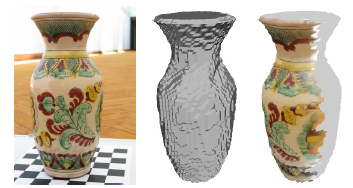
\includegraphics{introduction.png}
	\caption{对一个花瓶的纹理映射示意图}
\end{figure}
\section*{5.2 算法综述}
\subsection*{5.2.1 基于马尔科夫随机能量场(Markov Random Field,MRF)的纹理映射}
定义三维模型的面片为$F_{1},F_{2}...F_{k}$,图片集的图片为$V^{1},V^{2}...V^{N}$,马赛克集合$M=\{m_{i},1\leq i\leq k,i \in Z\}$,其中$m_{i}$意为面片$F_{i}$的像素由图片$V_{m_{i}}$映射而成。\\
定义$w_{i}^{j}$为把图片$V^{j}$映射回面片$F_{i}$上的代价函数,一种常见的定义方法是

\begin{align} w_{i}^{j} = sin\phi^{2}	\end{align} $\phi$是拍摄图片$V^{j}$时,相机正对的方向向量和面片$F_{i}$的法向量的夹角。那么整个三维模型的自映射代价就为
\begin{align} E_{Q}(M) = \sum_{1}^{K} w_{i}{m_{i}}	\end{align}

而只有自映射代价是不够的:如果两个面片相邻,但是他们用不同的图片进行映射,就可能产生缝隙。为了尽可能减少缝隙,我们定义互映射代价函数
\begin{align} E_{S}(M) = \sum_{\{i,j\}^{}\in N} w_{i,j}^{m_{i},m_{j}} 	\end{align}
$\{i,j\} \in N$意为$F_{i},F_{j}$两面片相邻,也就是有公共边。其中,
\begin{align} w_{i,j}^{m_{i},m_{j}}=\int_{E_{ij}}^{}D_{m_{i},m_{j}}(X)dX	\end{align}

$E_{ij}$是$F_{i},F_{j}$的公共边,$D_{m_{i},m_{j}}(X)$是三维模型上的点X在$V^{m_{i}},V^{m_{j}}$两个图片上的投影像素的RGB差值(欧几里得距离)。\\
这样就可以定义总的代价函数为

 \begin{align}  E(M)=E_{Q}(M)+\lambda E_{S}(M)	\end{align}

$\lambda$是一个参数。那么这一步就可以转化成一个优化问题:求马赛克集合M,使得代价函数E(M)最小。我们使用图割算法($\alpha$-expansion Graph Cut)实现这一步,详见5.3.1。

 \begin{align} M=argmin_{M}E(M) 	\end{align}
也就是找到每个面片的映射图片,使得总共的映射代价最小。
\subsection*{5.2.2 消除纹理缝隙的方法}
我们使用缝隙平整(Seam Leveling)方法来消除上一步还残留的缝隙。\\
我们先将所有的面片划分成若干个连通块$C_{1},C_{2},...C_{T}$,每个连通块的面片是连通的,而且在上一步得到的马赛克值相同。\\
我们定义强度函数$f_{i}{j}$为连通块$C_{j}$在点$V_{i}$的RGB值,前提是点$V_{i}$周围有面片属于连通块$C_{j}$。之后我们尝试求得一个补充强度函数$g_{i}{j}$,使得f+g对应的纹理没有缝隙。\\
定义集合M为所有使得点$V_{i}$周围有面片属于连通块$C_{j}$的数对(i,j)构成的集合,集合L为所有使得点$V_{i},V_{j}$相邻的数对(i,j)构成的集合,那么我们可以定义关于f,g的能量函数如下:
 \begin{align} 
 	\sum_{\substack{(i_{1},j)\in M \\ (i_{2},j)\in M \\ (i_{1},i_{2})\in L}} (g_{i_{1}}^{j}-g_{i_{2}}^{j})^{2}+\lambda \sum_{\substack{(i_{1},j)\in M\\(i_{2},j)\in M}}(g_{i}^{j_{1}}-g_{i}^{j_{2}}-(f_{i}^{j_{2}}-g_{i}^{j_{1}}))^{2}	\end{align}
 其中参数$\lambda$是一个100左右的大数字。这是一个典型的最小二乘问题,可以用高斯-牛顿迭代法求解,具体求解方法见5.3.2。
 \begin{figure}[h]
 	\centering
 	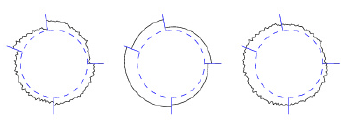
\includegraphics{seam.png}
 	\caption{缝隙平整(Seam Leveling)方法的示意图}
 \end{figure}
 \section*{5.3 具体求解方法}
\subsection*{5.3.1 图割算法}
图割算法($\alpha$-expansion Graph Cut)是上文第一部分的解决方法。\cite{name3}我将从代价函数求解,建图,整体步骤,网络流具体求解四个部分来介绍这个算法在本内容中的应用。
\subsubsection*{代价函数求解}
求解自映射代价函数和互映射代价函数的方法很简单,分别参考公式(1)(2)和(3)(4)就可以了。其中要注意的一点是,如果在某张图片$V_{i}$的角度看不到面片$F_{j}$,那么应该设置自映射代价为无穷。这就需要判断是否可见了。这里提供一种应用OpenGL的参考方法。\\
假如要判断在某张图片$V_{i}$的角度能否看得到面片$F_{j}$,可以先判断这个面片的顶点是否有可见的。可以先把原始模型输入进OpenGL里,然后给每个顶点赋不同的颜色,然后设置观测角度为拍摄这张图片的角度,这样就能得到一张投影图片。然后遍历这张投影图片就可以确定在这个视角中,哪些点是可见的。\\
 \begin{figure}[h]
	\centering
	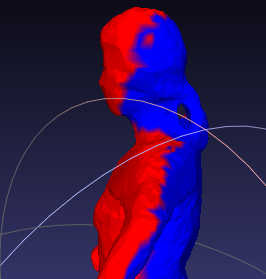
\includegraphics{cansee.png}
	\caption{判断从人的正面看,人的某些部分是否可见的结果示意图。红色的面片可见,蓝色不可见}
\end{figure}
\subsubsection*{图割算法的建图}
假设当前要更新图片$V_{i}$,此时的马赛克为M,那么建图规则如下:\\
有一个源点$\alpha$和一个汇点$\overline{\alpha}$,每个面片对应一个顶点,还需要按照需要添加若干辅助节点。\\
对于面片$F_{j}$,源点到其对应点p的边权$t_{p}^{\alpha}=D_{p}(\alpha)$,意为如果这个面片选用当前更新的图片$V_{i}$进行映射,产生的自映射代价。\\
同样,对于面片$F_{j}$,如果其马赛克值不等于i,也就是这个面片对应的图片不是当前更新的图片$V_{i}$,则其对应点到汇点p的边权$t_{p}^{\overline{\alpha}}=D_{p}(f_{p})$,意为这个面片使用自己马赛克的图片进行映射,产生的自映射代价。否则边权就是无穷大。\\
对于两个相邻面片$F_{m},F_{n}$和其对应点p,q,如果这两个面片马赛克值相等,也就是用同一张图片进行映射,那么p到q就不需要辅助节点,可以直接相连,边权为$V_{\{p,q\}}(f_{p},\alpha)$,意为图片$F_{m}$使用其自己马赛克的图片进行映射,而图片$F_{n}$使用当前更新的图片进行映射,双方产生的互映射代价。\\
如果这两个面片马赛克值不相等,也就是使用不同的图片进行映射,那么就需要添加辅助节点a。p到a的边权为$e_{\{p,a\}}=V_{\{p,q\}}(f_{p},\alpha)$,a到q的边权为$e_{\{a,q\}}=V_{\{p,q\}}(\alpha,f_{q})$,含义和上面一致。而辅助节点a到汇点也有边,权重为$t_{a}^{\overline{\alpha}}=V_{\{p,q\}}(f_{p},f_{q})$,意为这两个面片都使用自己的马赛克图片进行映射产生的互映射代价。\\
 \begin{figure}[h]
	\centering
	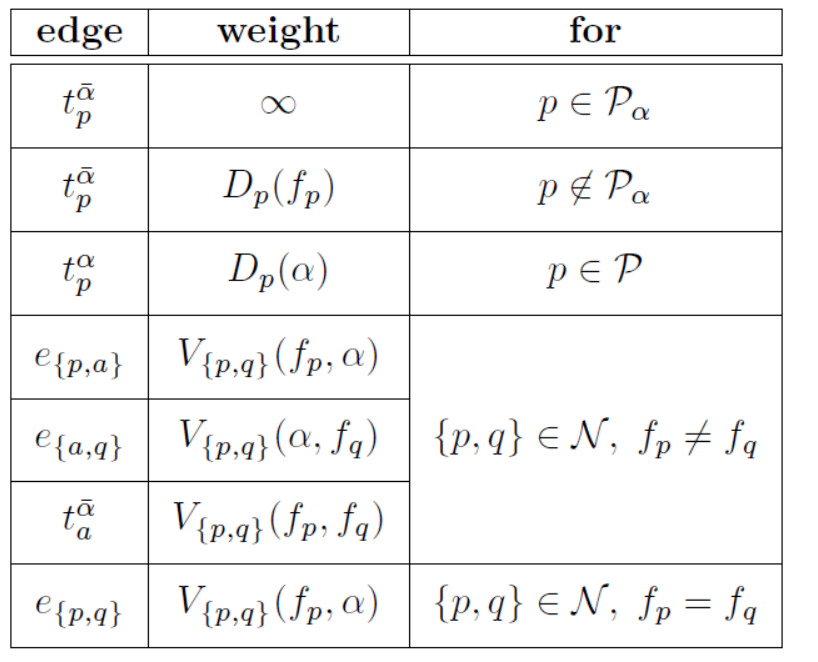
\includegraphics[scale=0.5]{cutmatrix.png}
	\caption{图割算法的具体建图方法}
\end{figure}
 \begin{figure}[h]
	\centering
	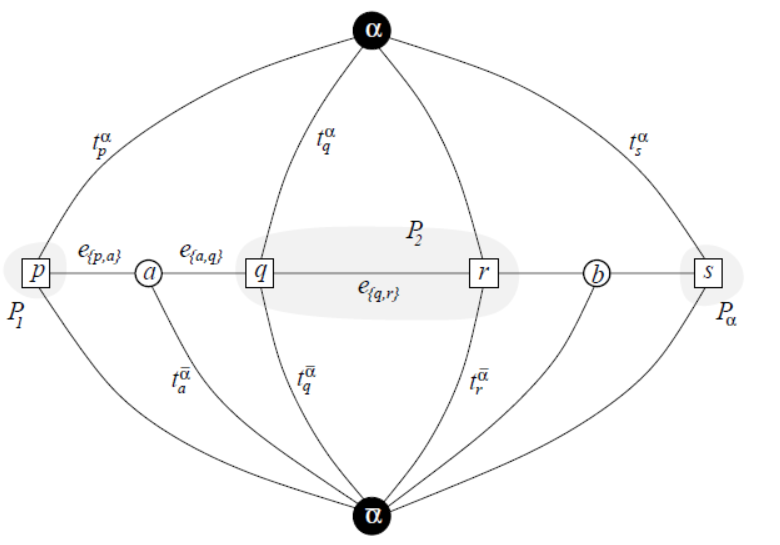
\includegraphics[scale=0.5]{cutshow.png}
	\caption{图割算法的图例}
\end{figure}
\subsubsection*{图割算法的流程}
、开始时可以设置每个面片的马赛克为随机值。\\
1.设置success为0\\
2.遍历每个图片$V_{i}$\\
2.1\qquad  按照上一段的方法,根据当前图片$V_{i}$和马赛克M建图。\\
2.2\qquad   用网络流算法求解出这个图的最小割。\\
2.3\qquad  更新马赛克值:对于这个图从源点$\alpha$到面片对应点p的边$t_{\alpha}^{p}$,如果这个边在最小割中,那么就设置p对应的面片的马赛克值为当前图片i。更新后要计算总权重,如果比之前求出的最小权重小,则这样更新是可行的。否则就不应该这样更新,要退回之前的马赛克值。如果进行了可行更新,就设置success为1。\\
3.如果success = 1,就回到1。否则结束,当前的马赛克值就是最优的。

\subsubsection*{网络流算法}
常见的网络流算法,比如Ford-Fulkerson算法,Dinic算法,预流推进等都可以求解这个问题,但是经过实验测试,这些算法求解都不如以下要介绍的算法快。\cite{name2}\\
这个算法可以分成三部分:求增广路径(grow),增加流量(augment),收集孤节点(adopt orphans)。为了实现算法,需要记录从属关系Tree(p),父子关系PARENT(p)。从属关系Tree定义如下:如果点p在从源点s开始的搜索树上,记为Tree(p)=S;:如果点p在从汇点t开始的搜索树上,记为Tree(p)=T;否则记为空。父子关系定义如下:如果p在搜索树S或T上,那么PARENT(p)就是搜索p的上一个节点,否则就是空。整体流程如下:\\
1.初始化源点集合S={s},汇点集合T={t},已激活集合A={s,t},孤节点集合O=$\emptyset$,以及从属关系Tree(p),父子关系PARENT(p)。\\
2.while true\\
2.1 \qquad 求增广路径(grow),找到一条从s到t的增广路径,如果找不到就结束\\
2.2 \qquad 沿这条增广路径增加流量(augment)\\
2.3 \qquad 收集孤节点(adopt orphans)\\
3.end while
\newpage
\paragraph*{求增广路径(grow)}-\\
1.while $A \ne \emptyset$\\
2.\qquad 从已激活集合A中选一个点p\\
3.\qquad 遍历所有p的可更新邻点q,要求是如果Tree(p)=S,则p到q的边未满。如果Tree(p)=T,则q到p的边非空。\\
3.1\qquad \qquad 如果Tree(q)=$\emptyset$,那么把q加入p所在的搜索树,使得Tree(q)=Tree(p),PARENT(q)=p,并且把q加入集合A\\
3.2\qquad\qquad 否则如果Tree(q)$\ne \emptyset$,那么此时就找到了一条s到t的可增广路。\\
4.\qquad 将点p移出集合A\\
5.end while
\paragraph*{增加流量(augment)}-\\
这一步只需要找到可增广路的瓶颈$\Delta$,也就是最多可增广的量,然后用$\Delta$去增广这条道路,使得正边流量增加$\Delta$,反边流量减少$\Delta$就可以了。\\
之后还要用这条可增广路上的饱和边(正边流量满,反边流量空)更新孤节点集合O:\\
如果Tree(p)=Tree(q)=S,那么设置PARENT(q)=$\emptyset$,将q加入孤节点集合O\\
否则如果Tree(p)=Tree(q)=T,那么设置PARENT(p)=$\emptyset$,将p加入孤节点集合O\\
\paragraph*{收集孤节点(adopt orphans)}-\\
1.while $O\ne \emptyset$ \\
2.从O中取出孤节点p,并且把p移除出O\\
3.给p找一个合适的父亲节点q,使得Tree(q)=Tree(p),q到p的边是可增广的(正边非满反边非空),而且q的祖先(用PARENT迭代求得)要么是源s要么是汇t。\\
3.1 \qquad 如果找到了这个父亲节点q,我们就让PARENT(p)=q就可以了\\
3.2 \qquad 如果没找到,就需要做如下操作:\\
3.2.1 \qquad \qquad 遍历p的所有邻点q\\
3.2.1.1 \qquad \qquad \qquad 如果q到p的边可增广(正边非满反边非空),就把q加入已激活点集A\\
3.2.1.2 \qquad \qquad \qquad 如果PARENT(q)=p,就设置PARENT(q)为$\emptyset$,并且将q加入孤节点集合P\\
3.2.2 \qquad \qquad TREE(p)设置为$\emptyset$,将p移除出已激活点集A\\
4.end while
 \begin{figure}[h]
	\centering
	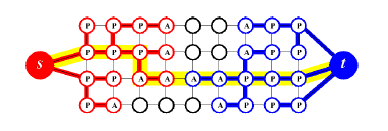
\includegraphics{networkflow.png}
	\caption{网络流方法示意图}
\end{figure}
\subsection*{5.3.2 缝隙平整算法的实现}
\subsubsection*{高斯-牛顿法的实现}%引用了博客https://www.cnblogs.com/leexiaoming/p/7257198.html
求解这种最小二乘法,比较好的方法就是高斯-牛顿迭代。我们令$g$为变量x,能量函数为函数F(x),令x初始为0,计算步骤如下:\\
1.求出当前的能量函数值F(x)和梯度J(x)\\
2.求解增量方程
 \begin{align} H\Delta x=s	\end{align}
 其中$H=J(x)^{T}J(x),s=-J(x)^{T}F(x)$\\
3.如果$\Delta x$足够小,则停止,否则用x+$\Delta x$更新x,回到1
\subsubsection*{求解增量方程的方法--共轭梯度法}%引用了博客https://blog.csdn.net/qq547276542/article/details/78186050
因为g的维度很大,对于几十万个面片模型,g有上千万维。这是典型的稀疏向量,稀疏矩阵的情形。直接求解这个增量方程必然计算量巨大,因此我们可以采用共轭梯度法来间接求解这个方程。\\
\paragraph{原理}
求解增量方程(8)等价于求解使得$||H\Delta x - s||$最小的$\Delta x$,也就是求解 $argmin(\frac{1}{2}\Delta x^{T}H^{T}H\Delta x - s^{T}H\Delta x)$。$H=J(x)^{T}J(x)$,显然为正定矩阵,这符合共轭梯度法的条件。\\
\paragraph{流程}
求解方程Ax=b的算法如下。根据共轭梯度法的性质,这个算法中相邻两次的r是正交的,可以用来检测是否正确。
在这里,矩阵A就是上文的H,b就是上文的s。具体实现这个算法可以用多线程库cuda中的cublas,cusparse两个包来实现。步骤如下图:
 \begin{figure}[h]
	\centering
	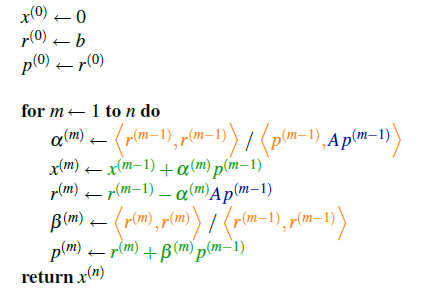
\includegraphics{conjugate.png}
	\caption{共轭梯度法的伪代码}
\end{figure}

\bibliography{reference}
\end{CJK}
\end{document}